% Remove 12pt, change draftcls -> final when doing final.
\documentclass[journal]{./IEEE/IEEEtran}
\usepackage{cite, graphicx}
\graphicspath{ {images/} }

\newcommand{\SPTITLE}{Room-8! - A Matchmaking Application for Finding College Roommates}
\newcommand{\ADVISEE}{Joseph Matthew R. Marcos}
\newcommand{\ADVISER}{Caroline Natalie M. Peralta}

\newcommand{\APPNAME}{Room-8! }
\newcommand{\BSCS}{Bachelor of Science in Computer Science }
\newcommand{\ICS}{Institute of Computer Science}
\newcommand{\UPLB}{University of the Philippines Los Ba\~{n}os }
\newcommand{\REMARK}{\thanks{Presented to the Faculty of the \ICS, \UPLB\
                            in partial fulfillment of the requirements
                            for the Degree of \BSCS }}

\markboth{CMSC 190 Special Problem, \ICS}{}
\title{\SPTITLE}
\author{\ADVISEE~and~\ADVISER
\REMARK
}
\pubid{\copyright~2016~ICS \UPLB}

%%%%%%%%%%%%%%%%%%%%%%%%%%%%%%%%%%%%%%%%%%%%%%%%%%%%%%%%%%%%%%%%%%%%%%%%%%

\begin{document}

% TITLE
\maketitle

% ABSTRACT
\begin{abstract}
    This article explores the role and significance of roommates in a college student's development - from the initial
    adaptation with the roommate setting, to their academic performance and life after college. The importance of
    finding the proper roommates so that a student can maximize their psychological development, get higher grades, and
    develop open-mindedness is highlighted. A solution is proposed in the form of a web application that can help \UPLB
    students find mutually beneficial roommates for their college life. This solution also extends itself to solve the
    dorm-finding problem students experience at the start of every semester.

\end{abstract}

% INDEX TERMS
\begin{keywords}
UPLB, University of the Philippines Los Ba\~{n}os, Roommate, Roommate matching
\end{keywords}

% INTRODUCTION
\section{Introduction}
% To be effective, the introduction should answer the questions ``Why and What For (Four)?" Expanded, these questions are----
% \subsection{Why is the topic of interest?}

    % Expound more on the psychological importance of college
    Several studies support that social functioning during college plays a major role in a student's psychological
    development. According to Chickering and Reisser, one of the seven vectors of psychological developmental issues
    that college students face is cultivating mature interpersonal relationships\cite{chickering}. College-aged students
    also fall within Arnett's emerging adulthood stage, where identity formation is associated with
    friendships\cite{erb}. According to Erikson's stage theory of psychological development, a young adult prefers to
    seek intimacy in relationships rather than in isolation\cite{erikson}. 

    Studies have linked social functioning to mental health and adjustment to college life \cite{erb}. A plethora of
    benefits such as psychological well-being, environmental mastery, personal growth, and self-acceptance have all been
    related to a student's ability to form meaningful relationships\cite{erb}. The conjunction between a person{'}s
    social capabilities and these benefits is so strong thatit can be used to predict how well the student will adjust
    to the new demands in college life. An individual who can develop good relationships in college has less problems
    \cite{erb}. 

    \subsection{Why College Roommate Relationships}
    The goal is to make it easier for students to acquire these benefits with less guess work. Students have to develop
    better interpersonal relationships in college $-$ particularly roommate relationships because these are
    relationships that are widely experienced by many college students\cite{erb}. Roommates have frequent contact,
    negotiations of responsibilities and compromises about the living environment, which often include noise level,
    cleanliness level, sleep/waking hours, visitors, decorations, and bills\cite{erb}. These may become challenges when
    dealing with each other. 

    For many college students, many {``firsts"} add to the challenges of campus life. Usually, roommates are the first
    {``people of equal status"} they live with, compared to the parent-child relationship they usually experience at
    home\cite{erb}.

    Unlike friendships, college students may often not choose roommates, causing personality mismatches. Many studies
    support that roommates, while having the potential to be a boon to a student, can also hinder a student from having
    a quality college life. According to Erb\cite{erb}, citing Liu\cite{liu}, in a 31,500 sample sized survey in the
    United States of America, 50.1\% of women and 44.1\% of men experienced “frequent” conflicts with roommates or
    housemates. In another survey in the same country, 5.6\% of undergraduates reported that difficulties with their
    roommates have hampered their academic endeavors\cite{erb}. For comparison, 4\% of American students said that
    alcohol did the same thing\cite{erb}.

    College roommates are targeted because it has been proven that college roommate relationships have a momentous
    effect on a student's performance before and after graduation. Although the college-roommate phenomenon has existed
    for a long time, there is only one paper that congregates empirical information about college-roommate
    relationships\cite{erb}. 

    \subsection{Proposed Solution}
    In order to maximize the number of compatible roommates on campus, a roommate-matching application will be made for
    UPLB. Unlike other roommate matching applications that exist today, the target of this application are students of
    \UPLB who are looking for roommates. These students have different needs and preferences to working class people, so
    existing roommate matching applications cannot be used. In addition, there are no roommate matching applications
    that cater to the UPLB area or the Philippines. It is about time that one is created for campus. The aim of this
    Special Problem is to create a proof of concept of an application that can generate initial pairings for roommates.


\pubidadjcol

    % Similar Applications
    \subsection{Similar Applications}
    There are existing roommate finding tools, which have more similarities than differences. They ask the user if they are
    looking for a place to stay, or if they have a room and are looking for someone to stay with them. Then, the user is
    bombarded with a long questionnaire that they have to fill out. It covers most of the basic criteria a person would have
    when looking for a room. The union of questions asked in both websites can be seen in the appendices. 

        % Both applications have similar questions, but have subtle insignificant differences. Roommates.com requires you to log
        % in even before you start filling out the questionnaire. Roommie Match does not. However, in order to get a match, you
        % will have to provide your credentials. Some people may find this surreptitious, as users will be forced togive their
        % credentials after they have already filled out a long form. 
        \subsubsection{Roommates.com}
        Roommate.com\cite{roommates.com} is a web application that caters to people looking for roommates in the United States
        of America. It can be accessed by going to \textit{www.roommates.com}. The home page enumerates cities where the
        application is most often used, such as Las Vegas, Houston, Atlanta, Los Angeles, New York, etc. 

        Users are required to create an account to use the service. Account creation is free regardless of your location. Among
        its listed features for free accounts include: photo profile, two-way matching, and the freedom to contact potential
        roommates. The application has a premium account option, which is required to read the messages sent to you by other
        users in the application. It costs \$5.99 for three days, roughly \$20 dollars for 30 days, and \$30 dollars for 60
        days. 

        Another feature of Roommates.com is the powersearch feature where the user can do searches with focused criteria. It is
        similar to Google's advanced search. The user will be redirected to a form that asks some questions (see appendix). Once
        the user has filled out the form, a list of matching roommates will appear. The user is able to see the profiles of the
        matched individuals, matching the information they wrote when creating an account. 

        The only way to contact a matched person is by sending them a message with the built in messaging system. Sending
        messages is free, but reading them requires a premium account. Therefore, you need to be a paying user to fully utilize
        Roommates.com.

        Roommates.com is not feasible for use in UPLB because there are no locations near the \UPLB that come up in the list of
        city selections. The form also forces the user to specify their state - a piece of information that is irrelevant for
        people living outside the United States of America. The website has a lot of JavaScript alerts and prompts when
        navigating, which is bad for user experience \cite{UX1}. Finally, a free user won't be able to get any utility out of it
        without paying.

        \subsubsection{Roommiematch.com}
        Roommiematch is another roommate match making web application that caters to some cities in Canada and the United States
        of America. Unlike Roommates.com, Roommiematch starts asking users about their preferences without requiring them to
        create an account. It also caters to fewer cities than Roommates.com.

        One of the strengths of Roommiematch.com over other web applications is that the forms are reviewed by actual humans
        before the pairing actually occurs. They claim that many of the registration forms get tossed, ensuring the legitimacy
        of its subscribers. Roommiematch also has a more modern user interface - it has a flat design, and elements are larger
        than those found in Roommates.com.

        Its weakness is that the registration process is so long and you cannot save your previous answers. It was composed of
        over ten multiple choice questions, and four questions where you had to type the answer. You have to answer all of them
        in one go.

        A feature that may both be good and bad is that here is no way to view the profiles of people you are matched with
        except through the emails they send you. The reasoning behind this is so that less of the work goes to the user and
        their users' information does not get published everywhere. There is no need to revisit the website time after time.
        They claim that this is the feature that deters scammers from even registering.

        Roomiematch can actually be considered a service that you subscribe to rather than an application. This is because there
        is no application you can interact with after filling out the form. Their team will email you updates every time you
        have a match, and it is up to you to contact your potential roommate. 

        \subsubsection{Tinder}
        Tinder is a mobile application in Android and iOS that has features that will be useful. It's purpose is not to match
        potential roommates, but to match potential dating partners. It is interesting because in 2015, it had an estimated 50
        million users\cite{tinderstat2}, 80\% of which were were millenials, or individuals born after 1982
        \cite{tinderstat}\cite{millenial}. It is intuitive to use, and has a use pattern that has been proven to be easily
        understood by millenials. This roommate matching application has to have a similar use-pattern to make it easier for the
        user. 

        When using Tinder, a user has to create an account. Tinder has the option of letting you log in with your Facebook
        account. Allowing Tinder to connect to your Facebook will allow it to get some data for your profile. There is an option
        to create an account without connecting it to Facebook. Once the account has been created, a user is prompted to fill
        out a few more fields, including a short description about oneself and a profile photo. The user can also make
        constraints that the application will consider when finding a match.

        Tinder is all about the pictures and description a user entered. The user is shown a list of other users that may
        interest them. For every entry, the user can swipe right if they is interested in being matched with the user, and left
        if not. If two people are interested in each other, Tinder matches them together and the two users can communicate.

    \subsection{The Ideal Roommate Matching application}
    The ideal roommate match-making application has to be similar to existing ones, but tailored in such a way that it
    caters to the interests of UPLB students. Modern user experience strategies have to be followed. Its features have
    to be planned well to make it more relevant than the previous applications mentioned.

    There are many papers that list the factors that facilitate friendship. However, most of them are dependent on what
    happens during the first meeting or interaction. Some of the criteria are subjective, such as honesty, which  vary
    from person to person. Other criteria cannot be controlled or measured with the application, such as honesty,
    virtues, and trustworthiness. Due to the lack of an empirical basis to measure these constructs, it can be predicted
    that not all matched roommates will be friends.

    There are a few elements of friendship chemistry that can be used to assess match people together. Friendship
    chemistry can be broken down into five main elements - namely reciprocal candor, mutual interest, personableness,
    similarity, and physical attraction\cite{f_chemistry}. Each of these elements can also be broken down and measured
    relatively well. When people were asked about these elements, it showed that people who experienced friendship
    chemistry were analogous\cite{f_chemistry} - which reflects other research that friends are people with many
    similarities\cite{similar}. They claimed to have nearly identical values and morals, and they understand each other
    well\cite{f_chemistry}. Agreeability between the parties is also a significant factor when predicting friendship
    chemistry \cite{f_chemistry}.

    A ideal roommate matchmaking application must be able to match users based on similarities. But it must still be
    able to match people who are not exactly identical.
    % Metrics for the ideal Roommate matchmaking application


% MATERIALS AND METHODS
\section{Methods}

\subsection{Architecture and Technologies}
The application will consist of a database, the server, and the client. A simplified version of the projected
architecture is shown below.

% Architecture diagram
\begin{figure}[h]
\centering
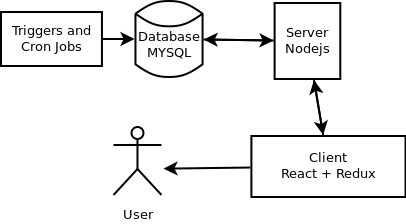
\includegraphics[scale=0.5]{Architecture}
\caption{This is the general architecture of the program. Technologies to be used are labelled appropriately}
\end{figure}

For the database management system (DBMS), MySQL will be used. It is a very versatile DBMS and is easy to set up in most
machines \cite{mysqlpage}. Its popularity is the result of its good documentation and support for any issues that may
arise \cite{mysqlpage}. The use of Database Triggers will be leveraged to run the recommender system - the part of the
application that does the initial recommendation of roommates. Since the application is model-heavy, complicated
transactions have to be performed, hence the need for stored procedures and stored functions. Such features have simple
to limiting implementations in NoSQL DBMS.

The application will be hosted with a Nodejs server with the Expressjs microframework. They were designed with user
productivity in mind without limiting scalability and expressiveness on the code. It is also good at handling IO events
from the user, as it is event driven, meaning you can focus on the application logic.

For the client side frameworks, Reactjs with Redux will handle the view. A flux architecture will be enforced because it
is common today. React is easy to use for this kind of system because its separation of concerns make it easy to
maintain (and develop). It claims to be faster because it applies minimal changes to the DOM everytime your data
changes. The User Interface will use MaterializeCSS because it is lightweight and simple.

\subsection{The Recommender System}
A recommender system is used by applications to predict information and offer content to its users\cite{katarya}.
Youtube, for example, uses a recommender system to suggest videos that a viewer might find interesting. Amazon uses a
recommender system to advertise products to different shoppers.

A recommender system will be used as part of the server that creates suggestions for roommates. This is the most
important part of the application. It should be able to rate the compatibility of a user against all other users, and
give a score based on how similar they are. The results of the recommender system will be shown to the user, who has the
liberty of \textit{accepting} or \textit{rejecting} the suggestions. If two users \textit{accept} each other, they have
the possibility of being matched - depending on the score they received. This recommender system will be unsupervised
and will run everytime a user modifies their account details, or a user creates an account.

\subsection{User workflow Pattern}

To use \APPNAME , the user must first create an account. The questions listed in the appendix are not going to be asked.
Instead, the user will be asked for their name, age, address, phone number, and email. After an account is created, the
user can sign in and use the application.

To actually get some pairings, the user must fill out their roommate preferences. These are broken down into seven
forms, listed down in the appendix. The user does not need to answer all of the questions in one go. The user's answers
will be the criteria used by the application to make initial matches. Each question has an option called ``Don't care".
This is the option selected by default. If it is selected, that question will not be considered as a constraint when
making the matchings.

The user also has to fill out the discovery settings. It contains three questions: \textit{How strict do you want us to
be when looking for a match?}, and \textit{Are you currently looking for a roommate?}. The first question can be
answerable by any integer from 1 - 100. It will serve as the threshold score when displaying matches for the user. The
second question is a flag. If it is set, the application will start searching for matches to present to the user. If it
is unset, the user will not show in anybody's list of matchings or pairings.

The matches will come as a list of profiles. Initially, the users cannot see the contact details of ``matched" people.
However, they can see the preferences and answers of their ``matches". If a match is interesting, a user can choose to
accept it or not, much like in Tinder where the user swipes left or right. As new users are being created, more matches
can come by. If two people accept each other, they are then paired.

Paired people can now see each others' contact details. They can also use the in-app chat system. These pairings will
come as a list ordered by the similarities of their profiles. New pairings can come up as people use the application.
Paired people can finalize the roommate pairing. This will unset their discovery setting of ``Are you looking for a
roommate". A user can see the profile of the person he/she is finalized with any time.

If a pair disagrees, they can choose to discard that pairing. The discarded pair will appear in the user's blacklist and
will not be matched. A user can remove blacklisted users.

\begin{figure}[h]
\centering
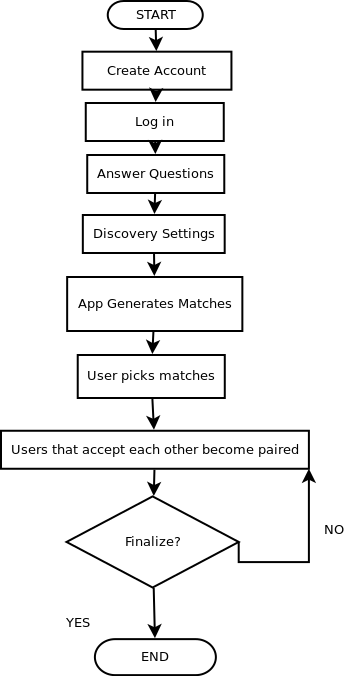
\includegraphics[scale=0.5]{Workflow}
\caption{This is the general workflow of your user}
\end{figure}
% Genyan na talaga ang arrow.

% How matches are scored
\subsection{How Matches are Scored}
In order to create potential matches, the compatibility between two users have to be measured. For the remainder of the
section, the user that needs a room will be called \textit{user1} and the user that has a room will be called
\textit{user2}. The algorithm initially gives each pair a score of zero. The application has 17 criteria for arbitrating
two users' compatibility. Each criteria in the questionnaire is worth a certain amount of points.  This scoring
algorithm will be applied to the cartesian product of the users that have a room and the users that are looking for a
room. The criteria as as follows:

    \subsubsection{Cleanliness}
        The cleanliness criterion is determined by 2 fields from each user:
        \begin{itemize}
                \item my\textunderscore cleanliness - A user's self-rating of their cleanliness level.
                \item preferred\textunderscore cleanliness - A user's preferred cleanliness level for their
                    potential roommate.
        \end{itemize}

        The preferred\textunderscore cleanliness of user1 will be compared to user2's my\textunderscore cleanliness and
        vice versa. A magnetism variable is assigned for each comparison, which can be computed as

        \begin{equation}
            magnetism_1 = 10-user1's\textunderscore cleanliness - user2's\textunderscore preference
        \end{equation}
        and
        \begin{equation}
            magnetism_2 = 10-user2's\textunderscore cleanliness - user1's\textunderscore preference
        \end{equation}

        The total cleanliness is the arithmetic mean of both magnetism variables

        $$score = (magnetism_1+magnetism_2)/2$$

    \subsubsection{Smoker}
        The smoking score is determined by comparing user1's smoking preference user2's smoking profile and vice versa.
        It is similar to the Cleanliness score in that it uses two variables from each user to determine the score.
        If user1's preference to a smoking partner is equal to user2's smoking profile, 5 is added to the score. If
        user2's preference to a smoking partner is equal to user1's smoking profile, another 5 is added. This criterion gives a
        maximum of 10 points.

    \subsubsection{Sex}
        The sex score is determined exactly the same way as the smoking score is determined.

    \subsubsection{Start Date}
        If user1's start date is greater than or equal to user2's start date, then it is implied that the room is
        available when user1 wishes to move in. If this is the case, this criterion will be given a score of 10.
        Otherwise, it returns a score of 0.

    \subsubsection{Rent Cost}
        The Rent Cost is a criterion used to determine whether or not a room is within a user's budget.
        The price range of user1's input is compared to user2's input for the rent cost. The variables that are
        considered are:
        \begin{itemize}
            \item rent\textunderscore start(user1) - User1's lower bound for rent cost.
            \item rent\textunderscore end(user1) - User1's upper bound for rent cost.
            \item rent\textunderscore cost(user2) - User2's monthly rent bill.
        \end{itemize}
        If the monthly rent of the room is within the range set by user1, then a score of 10 is given to this criterion.
        Otherwise, it is scored a 0.

    \subsubsection{Nearby Restaurants}
        A user looking for a room is given the option whether or not they prefer that there exists some nearby
        restaurant in their future temporary abode in UPLB. On the other hand, the user who has a room is asked whether
        or not there exists some nearby restaurant near their room. If user1 answers no, then it does not matter whether
        or not there is a nearby restaurant to the room, and a score of 10 is given. If user1 answers a yes, then a
        score of 10 will be given if user2 similarly answers yes. Otherwise, a score of 0 is given.

    \subsubsection{Travel Time to UPLB}
        This criterion is filled out by the user as the number of minutes it takes for a user to reach UPLB.
        If user1's answer is greater than or equal to user2's answer, then a score of 10 is given. Otherwise, a score of
        0 is given. 

        When user1's value is greater than or equal to user2's answer, it means that user1 is willing to settle for a
        longer travel time than what exists in user2's room.

    \subsubsection{General Location}
        This criterion is used to match the general location of both users. The users' entries for general location are
        then fuzzy matched to check how similar the user entrues are. The fuzzy matching returns a number as a percent
        of 100. That percentage match is multiplied as a percent of 10 and is returned as the score. A 100\% match is
        given a score of 10.

    \subsubsection{Utilities Cost}
        The Utilities Cost is a criterion used to determine whether or not a room is within a user's budget.

        The user looking for a room is asked whether or not it is acceptable for their potential room to charge their
        utility bills exclusive of the rent cost. If it is acceptable, then they are prompted for a price range they are
        willing to settle with.  The price range of user1's input is compared to user2's input for the rent cost. The
        variables that are considered are:
        \begin{itemize}
            \item utilities\textunderscore start(user1) - User1's lower bound for utilities cost.
            \item utilities\textunderscore end(user1) -  User1's upper bound for utilities cost.
            \item utilities\textunderscore cost(user2) - User2's monthly utilities bill.
        \end{itemize}
        If user2's answer is ``No", then a score of 10 is given".
        If user2's answer is ``Yes", and user1's answer is ``No", then a score of 0 is given.
        If both users answer ``Yes", then a score of 10 is given only if the monthly utilities bill of the room is
        within the range set by user1, then a score of 10 is given to this criterion.
        Otherwise, a score of 0 is given.

    \subsubsection{Utilities}
        This criterion is used check which utilities are available in the establishment. There are many subcriteria that
        constitute the total score of this criterion, namely:
        \begin{enumerate}
            \item Airconditioning
            \item Laundry
            \item Cooking
            \item Gas Stove
            \item Electric Stove
            \item Microwave
            \item Water Kettle
            \item Internet
            \item Torrenting
        \end{enumerate}

        For each of the aforementioned subcriteria, a score of 10 is added if user1's answer is equal to user2's answer.
        An answer of 'Do not care' awards a score of 10 for that subcriterion.


    \subsubsection{Speed}
        This criterion is only used if user1 or user2 selects ``Yes" for the internet subcriterion in the
        Utilities criteria. This criterion compares the internet speed requirement of both users. A score of 10 is
        given if user2's answer is greater than or equal to user1's answer because it means that the room is able to
        provide for the internet speed requirement of user1.

    \subsubsection{Study Time}
        This criterion determines whether or not the potential roommates study at the same time of the day. This is in
        hopes to provide a cordial understanding when lights and sounds should be turned off.

        The users are given the options of Morning, Evening, Both, Do not care. If either one of the users answers ``Do
        not care", it is assumed that the user is willing to adjust to the study habits of the other user. For such a
        situiation, a score of 10 will be given. Otherwise, a score of 10 will only be given if both users have exactly
        the same answer.

    \subsubsection{Guests in Room}
        Some people prefer to have freedom when allowing guests to enter their room, usually for projects and bonding
        time.

% Gale-Shapley's Algorithm
\subsection{Gale-Shapley's Algorithm in Room-8!}
Gale-Shapley's Algorithm is used to match two elements from different sets. It solves what is commonly known as the
Stable Marriage problem. It was introduced by Gale and Shapley when they were trying to assign aspirants to
universities, while considering their preferences and the preferences of the university\cite{irving}. The result of this
algorithm is a set of stable one-to-one correspondences between the two sets. A stable match is a match where there is
no pair of users that both prefer each other but are unmatched\cite{marriage}. In this application, the input of this
algorithm will be the initial scores of user groups (People who have a room and people without a room). Each user in
both groups has an ordered list of users from the other group that are sorted by their score from the matching
algorithm. The output will be the list of stable matches between the two groups.

User pairings whose matching score is below the threshold will not be considered by the algorithm. This means that the
matching is unacceptable. Gale-Shapley's algorithm allows this\cite{marriage}.




% \section{Proof of methods down here}

% RESULTS AND DISCUSSION
% \section{Results and Discussion}

% CONCLUSION AND FUTURE WORK
% \section{Conclusion and Future Work}

\newpage
% ACKNOWLEDGMENT
\section*{Acknowledgment}
I would like to thank my adviser \ADVISER for her patience. Without it, this entire project would not be realized.
% BIOGRAPHY
\begin{biography}[{
\includegraphics{./yourPicture.eps}}]{\ADVISEE}
    Matthew is a programmer that loves to solve real world problems. As a student of UPLB, he became interested in creating
    web applications that remedies the daily problems Filipinos experience. On his free time, he likes studying new
    technologies and reading books on history, technology, and the sciences. He is a fan of sci-fi books like those by
    Michael Crichton, and Douglas Preston and Lincoln Child.
\end{biography}


\newpage
% BIBLIOGRAPHY
% \bibliography{./cs190-ieee}
\bibliographystyle{./IEEE/IEEEtran}
\bibliography{marcoscmsc190sp}
% \nocite{*}

\newpage
% APPENDICES
\appendices
% Please look at the IEEE guidelines
\section{Some Roommate.com and Roommiematch.com questions} %Mandatory title to specify an appendix
\begin{enumerate}
    \item Are you looking for a room?
    \begin{itemize}
        \item I am looking for a room
        \item I have a room available for rent
        \begin{itemize}
            \item Current household composition (How many people currently living there)
            \item Furnishing of dwelling
            \item Parking availability
            \item Does the room have its own bathroom
            \item Additional amenities (See to match to questions enumerated below)
        \end{itemize}
    \end{itemize}
    \item Who you are looking for
    \begin{itemize}
        \item Straight female
        \item Professional
        \item Non Smoker
        \item Lesbian
        \item Student
        \item Smoker
        \item Straight male
        \item Unemployed
        \item Outside Smoker
        \item Gay male
        \item Military
        \item Retired
    \end{itemize}
    \item Age range
    \item Who
    \begin{itemize}
        \item Needs a place to live
        \item Has a place available
    \end{itemize}
    \item Location
    \begin{itemize}
        \item State
        \item City
    \end{itemize}
    \item Available (Date the room is available or the roomate is available to move)
    \item Payment (price range)
    \item Cleanliness
    \begin{itemize}
        \item Average
        \item Clean
        \item Messy
    \end{itemize}
    \item Pets
    \begin{itemize}
        \item No dogs
        \item No cats
        \item No caged pets
    \end{itemize}
    \item Whether or not you have a preference regarding children in the home
\end{enumerate}

% Room-8! Questions - To be updated more when we have more research on optimal roommate traits
\section{Questions and their Category in Room-8!}
\begin{enumerate}

    \item What are you looking for?
    \begin{itemize}
        \item A place with vacancies
        \item I have a room with vacancies
    \end{itemize}

    \item When
    \begin{itemize}
        \item Summers only?
        \item Start date?
        \item Duration of stay?
    \end{itemize}

    \item Utilities
    \begin{itemize}
        \item Air conditioning?
        \item Can I do my own laundry?
        \begin{itemize}
            \item Is there a washing machine?
            \item Is there a dryer?
            \item Is there a place to dry my clothes?
        \end{itemize}
        \item Can I cook? (Check all that apply)
        \begin{itemize}
            \item Gas Stove
            \item Electric Stove
            \item Microwave oven
            \item Water kettle
        \end{itemize}
        \item Internet connection
        \begin{itemize}
            \item What is the minimum speed requirement?
            \item Do you torrent?
        \end{itemize}
    \end{itemize}

    \item Hobbies
    \begin{itemize}
        \item Are you a gamer?
        \item Are you an activist?
        \item Are you into sports
    \end{itemize}

    \item Lifestyle
    \begin{itemize}
        \item Are you religious? / Are you a part of a cult?
        \item Do you urinate on the shower?
        \item What is an acceptable noise level for you? (1 - 10)
        \item Do you drink Alcohol?
        \item Do you smoke?
        \item Do you prefer to study in the early mornings or evenings?
        \item Do you have guests?
        \item Are you willing to share a bathroom?
        \item Do you have guests come over?
        \item Do you live with pets?
        \begin{itemize}
            \item Small caged animals (birds, hamsters)
            \item Not small caged animals (dogs)
        \end{itemize}
        \item Are you willing to share a bathroom?
    \end{itemize}

    \item Location Preferences
    \begin{itemize}
        \item Nearby Restaurants? (5 minute walk)
        \item How far from UPLB (How long a walk)
        \item General Area (List Barangays)
    \end{itemize}

    \item Misc
    \begin{itemize}
        \item Study area for guests?
        \item Easily Accessible
        \item Cost
        \item Payment scheme
        \item Curfew
    \end{itemize}
\end{enumerate}

\end{document}
